


\tikzset{every picture/.style={line width=0.75pt}} %set default line width to 0.75pt        

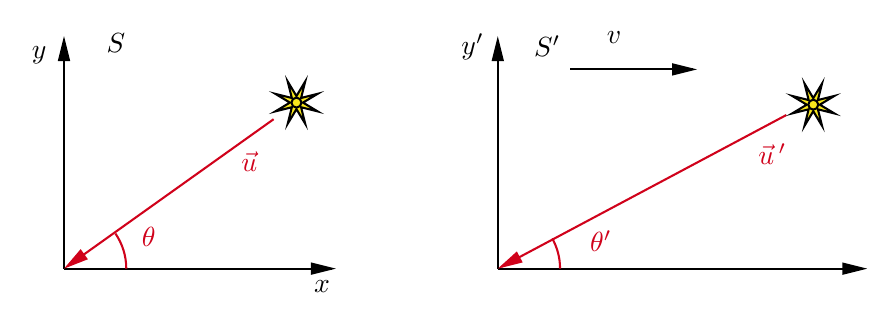
\begin{tikzpicture}[x=0.75pt,y=0.75pt,yscale=-1,xscale=1]
%uncomment if require: \path (0,159); %set diagram left start at 0, and has height of 159

%Straight Lines [id:da9890094660806119] 
\draw    (50,131) -- (179,131) ;
\draw [shift={(181,131)}, rotate = 180] [fill={rgb, 255:red, 0; green, 0; blue, 0 }  ][line width=0.08]  [draw opacity=0] (12,-3) -- (0,0) -- (12,3) -- cycle    ;
%Straight Lines [id:da08690688749783182] 
\draw    (50,131) -- (50,21) ;
\draw [shift={(50,19)}, rotate = 90] [fill={rgb, 255:red, 0; green, 0; blue, 0 }  ][line width=0.08]  [draw opacity=0] (12,-3) -- (0,0) -- (12,3) -- cycle    ;
%Straight Lines [id:da2482586897052299] 
\draw    (259,131) -- (435,131) ;
\draw [shift={(437,131)}, rotate = 180] [fill={rgb, 255:red, 0; green, 0; blue, 0 }  ][line width=0.08]  [draw opacity=0] (12,-3) -- (0,0) -- (12,3) -- cycle    ;
%Straight Lines [id:da8615500876857782] 
\draw    (259,131) -- (259,21) ;
\draw [shift={(259,19)}, rotate = 90] [fill={rgb, 255:red, 0; green, 0; blue, 0 }  ][line width=0.08]  [draw opacity=0] (12,-3) -- (0,0) -- (12,3) -- cycle    ;
%Straight Lines [id:da5227777052860076] 
\draw    (294,35) -- (353,35) ;
\draw [shift={(355,35)}, rotate = 180] [fill={rgb, 255:red, 0; green, 0; blue, 0 }  ][line width=0.08]  [draw opacity=0] (12,-3) -- (0,0) -- (12,3) -- cycle    ;
%Straight Lines [id:da2597202521855466] 
\draw [color={rgb, 255:red, 208; green, 2; blue, 27 }  ,draw opacity=1 ]   (151,59) -- (51.63,129.84) ;
\draw [shift={(50,131)}, rotate = 324.52] [fill={rgb, 255:red, 208; green, 2; blue, 27 }  ,fill opacity=1 ][line width=0.08]  [draw opacity=0] (12,-3) -- (0,0) -- (12,3) -- cycle    ;
%Straight Lines [id:da9851911945114264] 
\draw [color={rgb, 255:red, 208; green, 2; blue, 27 }  ,draw opacity=1 ]   (398,57) -- (260.77,130.06) ;
\draw [shift={(259,131)}, rotate = 331.97] [fill={rgb, 255:red, 208; green, 2; blue, 27 }  ,fill opacity=1 ][line width=0.08]  [draw opacity=0] (12,-3) -- (0,0) -- (12,3) -- cycle    ;
%Shape: Arc [id:dp19077533539300617] 
\draw  [draw opacity=0] (74.76,114.06) .. controls (78.07,118.88) and (80,124.71) .. (80,131) -- (50,131) -- cycle ; \draw  [color={rgb, 255:red, 208; green, 2; blue, 27 }  ,draw opacity=1 ] (74.76,114.06) .. controls (78.07,118.88) and (80,124.71) .. (80,131) ;  
%Shape: Arc [id:dp2171384210035181] 
\draw  [draw opacity=0] (285.23,116.43) .. controls (287.63,120.74) and (289,125.71) .. (289,131) -- (259,131) -- cycle ; \draw  [color={rgb, 255:red, 208; green, 2; blue, 27 }  ,draw opacity=1 ] (285.23,116.43) .. controls (287.63,120.74) and (289,125.71) .. (289,131) ;  
%Shape: Star [id:dp5969977180461878] 
\draw  [fill={rgb, 255:red, 248; green, 231; blue, 28 }  ,fill opacity=1 ] (166.21,40.84) -- (164.23,48.77) -- (172.16,46.79) -- (165.15,51) -- (172.16,55.21) -- (164.23,53.23) -- (166.21,61.16) -- (162,54.15) -- (157.79,61.16) -- (159.77,53.23) -- (151.84,55.21) -- (158.85,51) -- (151.84,46.79) -- (159.77,48.77) -- (157.79,40.84) -- (162,47.85) -- cycle ;
%Shape: Circle [id:dp8977056295728778] 
\draw  [fill={rgb, 255:red, 248; green, 231; blue, 28 }  ,fill opacity=1 ] (159.6,51) .. controls (159.6,49.67) and (160.67,48.6) .. (162,48.6) .. controls (163.33,48.6) and (164.4,49.67) .. (164.4,51) .. controls (164.4,52.33) and (163.33,53.4) .. (162,53.4) .. controls (160.67,53.4) and (159.6,52.33) .. (159.6,51) -- cycle ;

%Shape: Star [id:dp3269411686827788] 
\draw  [fill={rgb, 255:red, 248; green, 231; blue, 28 }  ,fill opacity=1 ] (415.21,41.84) -- (413.23,49.77) -- (421.16,47.79) -- (414.15,52) -- (421.16,56.21) -- (413.23,54.23) -- (415.21,62.16) -- (411,55.15) -- (406.79,62.16) -- (408.77,54.23) -- (400.84,56.21) -- (407.85,52) -- (400.84,47.79) -- (408.77,49.77) -- (406.79,41.84) -- (411,48.85) -- cycle ;
%Shape: Circle [id:dp7050666190258112] 
\draw  [fill={rgb, 255:red, 248; green, 231; blue, 28 }  ,fill opacity=1 ] (408.6,52) .. controls (408.6,50.67) and (409.67,49.6) .. (411,49.6) .. controls (412.33,49.6) and (413.4,50.67) .. (413.4,52) .. controls (413.4,53.33) and (412.33,54.4) .. (411,54.4) .. controls (409.67,54.4) and (408.6,53.33) .. (408.6,52) -- cycle ;


% Text Node
\draw (169,135.4) node [anchor=north west][inner sep=0.75pt]    {$x$};
% Text Node
\draw (33,22.4) node [anchor=north west][inner sep=0.75pt]    {$y$};
% Text Node
\draw (240,16.4) node [anchor=north west][inner sep=0.75pt]    {$y'$};
% Text Node
\draw (275,17.4) node [anchor=north west][inner sep=0.75pt]    {$S'$};
% Text Node
\draw (69,16.4) node [anchor=north west][inner sep=0.75pt]    {$S$};
% Text Node
\draw (310,15.4) node [anchor=north west][inner sep=0.75pt]    {$v$};
% Text Node
\draw (86,109.4) node [anchor=north west][inner sep=0.75pt]  [color={rgb, 255:red, 208; green, 2; blue, 27 }  ,opacity=1 ]  {$\theta $};
% Text Node
\draw (302,111.4) node [anchor=north west][inner sep=0.75pt]  [color={rgb, 255:red, 208; green, 2; blue, 27 }  ,opacity=1 ]  {$\theta '$};
% Text Node
\draw (134,73.4) node [anchor=north west][inner sep=0.75pt]  [color={rgb, 255:red, 208; green, 2; blue, 27 }  ,opacity=1 ]  {$\vec{u}$};
% Text Node
\draw (383,69.4) node [anchor=north west][inner sep=0.75pt]  [color={rgb, 255:red, 208; green, 2; blue, 27 }  ,opacity=1 ]  {$\vec{u}\,'$};


\end{tikzpicture}